\documentclass[12pt]{article}

\usepackage{amsmath}
\usepackage{graphicx}
\usepackage{subfigure}
\usepackage{float}
\usepackage{ulem}
\usepackage{bm}
\usepackage{anysize}
\usepackage{pythonhighlight}

\marginsize{2cm}{2cm}{0.9cm}{1.8cm}

\title{EECE 5639 Computer Vision\\ [2ex] \begin{large} Homework \#2 \end{large} }
\author{Jiyu Tian}
\date{}

\begin{document}
\maketitle
%%---------------------------------------------------------------
%% Question 1
%%---------------------------------------------------------------
\section{Solution:}
As shown in Figure \ref{raw}, the estimated noise of generated images is 1.9462, which is very approximate to 2, the targeted $\sigma$. And the worst case acquisition noise is 4.0258, around $2\sigma$.
\begin{figure}[H]
\centering
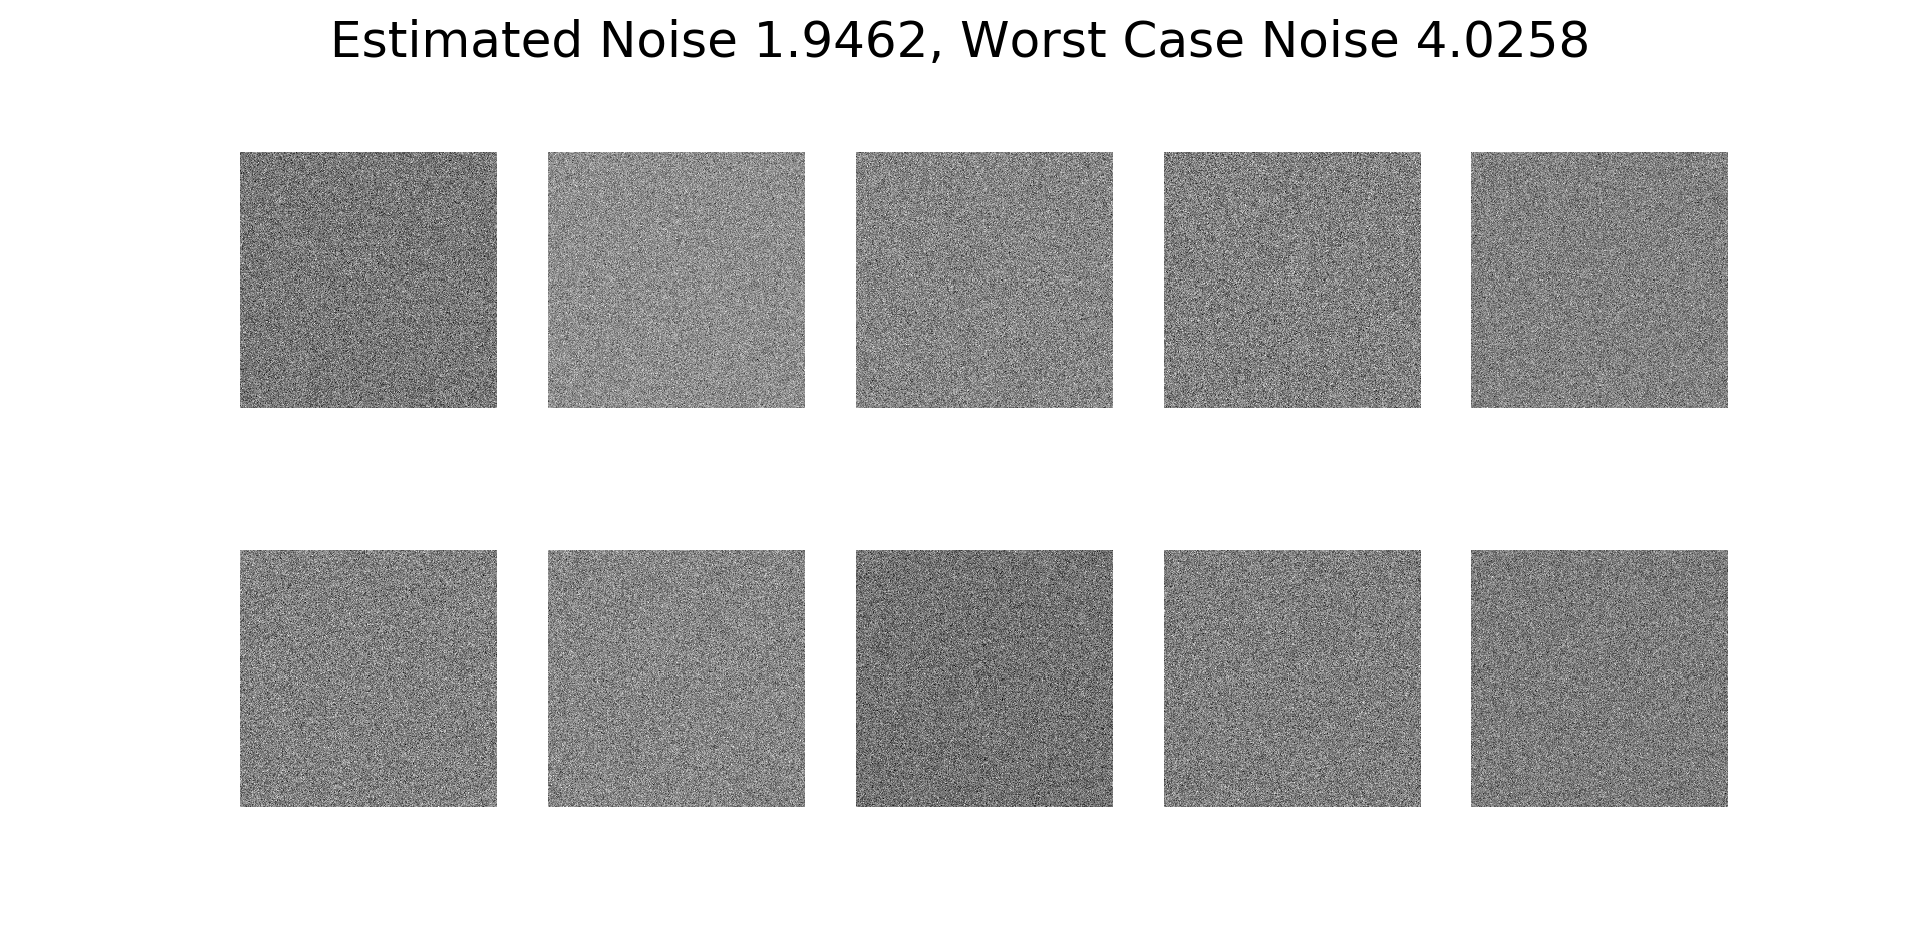
\includegraphics[width = 1\textwidth]{fig1.png}
\caption{Raw Images}
\label{raw}
\end{figure}
%%---------------------------------------------------------------
%% Question 2
%%---------------------------------------------------------------
\section{Solution:}
As shown in Figure \ref{filtered}, the estimated noise of the images after $3\times3$ box filter is 0.6472, and the worst case acquisition noise is 1.3971. Compared to the original ones, the image noises are reduced significantly, which we can also easily tell from the two figures.
\begin{figure}[H]
\centering
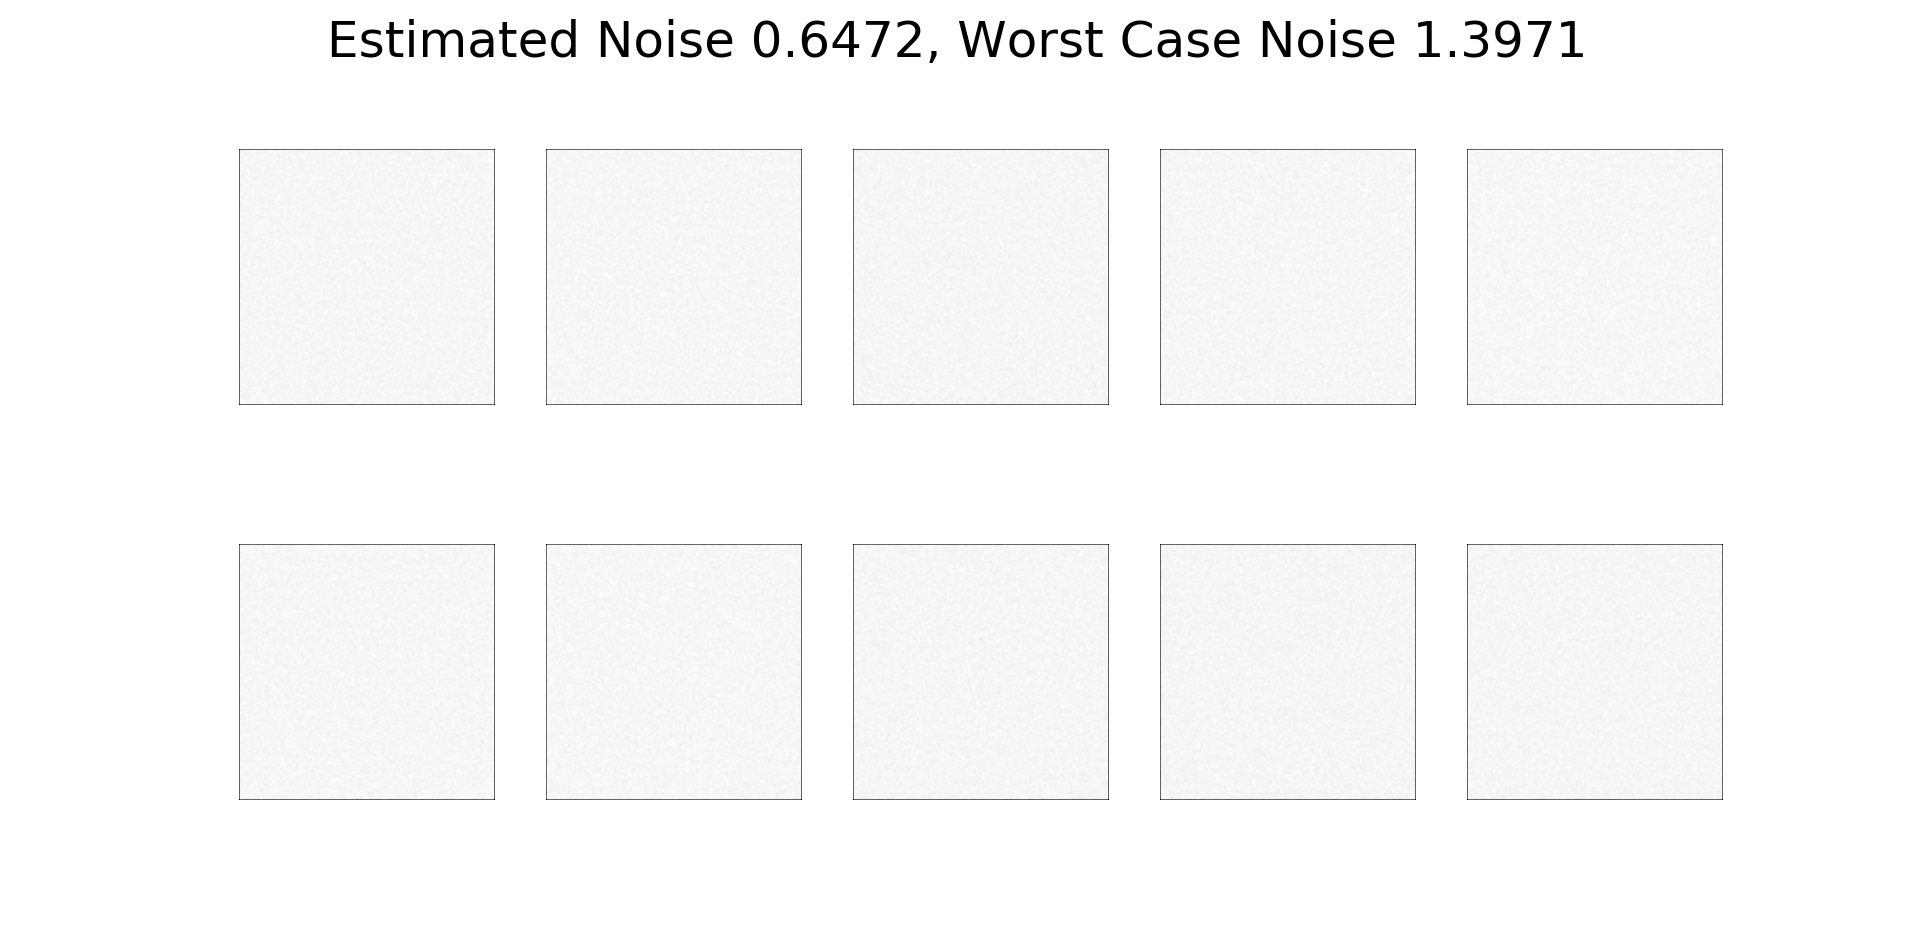
\includegraphics[width = 1\textwidth]{fig2.png}
\caption{Raw Images}
\label{filtered}
\end{figure}
%%---------------------------------------------------------------
%% Question 3
%%---------------------------------------------------------------
\section{Solution:}
The 2D Gaussian filter mask can be expressed as:
\begin{equation*}
    G(x,y) = \frac{1}{2\pi\sigma^2}e^{-\frac{x^2+y^2}{2\sigma^2}}
\end{equation*}
which can also be separated into two 1D Gaussian filters:
\begin{equation*}
    G(x) = \frac{1}{\sqrt{2\pi}\sigma}e^{-\frac{x^2}{2\sigma^2}}, G(y) = \frac{1}{\sqrt{2\pi}\sigma}e^{-\frac{y^2}{2\sigma^2}}
\end{equation*}
With implementation in python, a $5\times 5$ 2D Gaussian filter mask with standard deviation $1.4$ can be applied onto the sample figure, as shown in Figure \ref{ouput}. Please refer to Appendix for detailed code.
\begin{figure}[H]
\centering
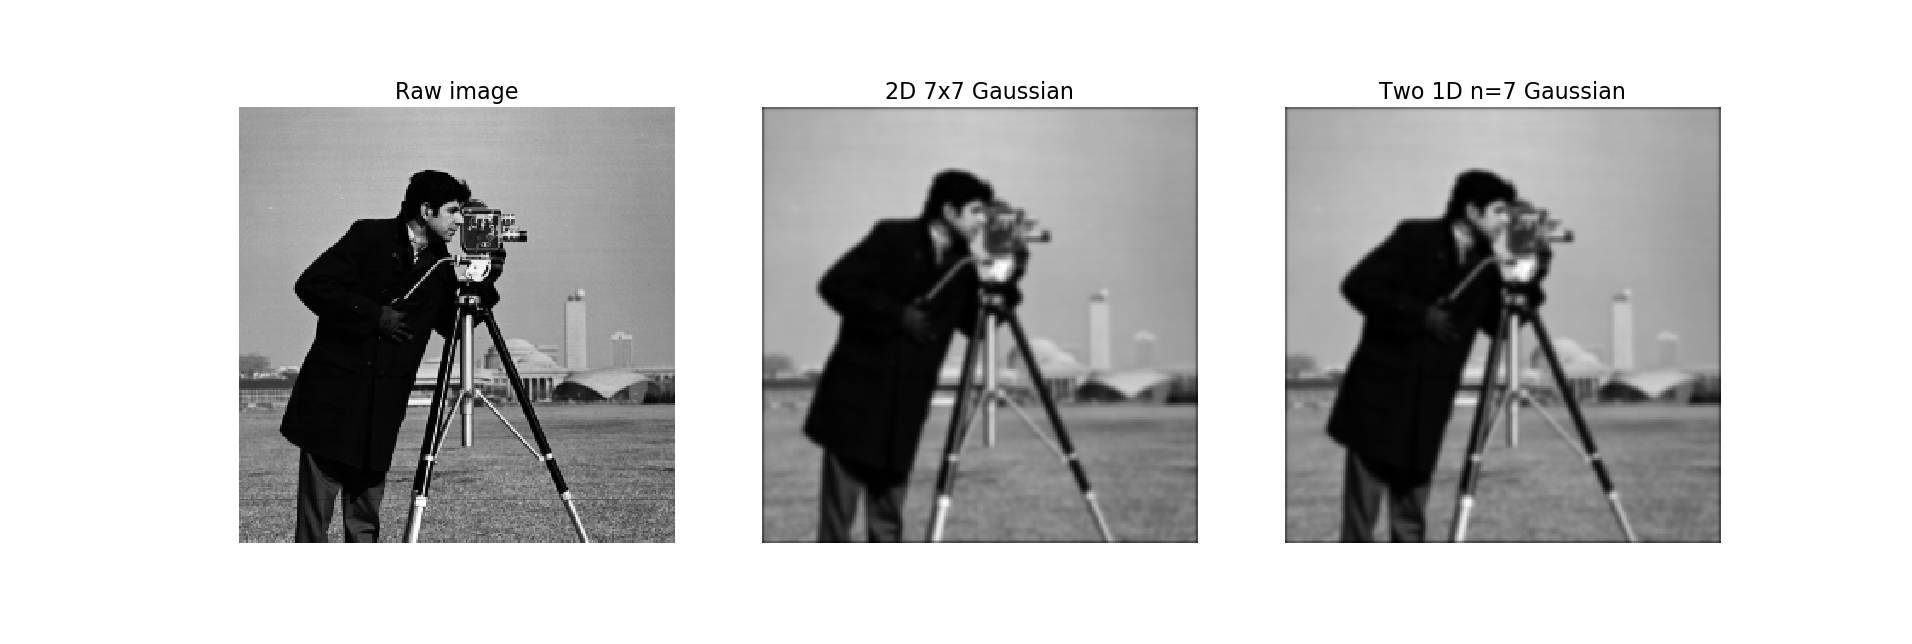
\includegraphics[width = 1\textwidth]{output.png}
\caption{Output of images after applying Gaussian filter mask}
\label{ouput}
\end{figure}

\vfill
\clearpage
%%---------------------------------------------------------------
%% Question 4
%%---------------------------------------------------------------
\section{Solution:}
(a) With filter (a): 
\begin{equation*}
{\left[ \begin{array}{cccccccccc}
6 & 8 & 10 & 16 & 22 & 28 & 34&  40 &  32& 24
\end{array} \right]}
\end{equation*}
\noindent With filter (b):
\begin{equation*}
{\left[ \begin{array}{cccccccccc}
7 & 9 & 10 & 13 & 19 & 31 & 37 & 40 & 36 & 28
\end{array} \right]}
\end{equation*}
\noindent (b) Consider a 1D image which is large enough to ignore the borders, with additive, uncorrelated Gaussian noise with zero mean and variance $\sigma^2$. Since filter (b) has different weights upon each filtered pixel, its computation cost is higher than that of filter (a). As for the variance of the noise, with filter (a), a pixel in the output noise $O$ with respect to input noise $I$ is:
\begin{equation*}
O_i = \frac{1}{5}\sum^2_{j = -2}I_{i+j}
\end{equation*}
The expected value of a pixel after filtering is:
\begin{equation*}
E[O] = E\left[\frac{1}{5}\sum^2_{j = -2}I_{i+j}\right] = \frac{1}{5}\sum^2_{j=-2}E\left[I_{i+j}\right] = 0
\end{equation*}
The variance of a pixel after filtering is:
\begin{equation*}
\begin{aligned}
E[(O-E[O])^2] &= E[O^2] \\
&= E\left[\frac{1}{25}\left(\sum^2_{j = -2}I_{i+j}\right)^2\right]\\
&= \frac{1}{25}E\left[\sum^2_{j-2}I^2_{i+j} + \sum^2_{m,n = -2}I_{i+m}I_{i+n}\right]\\
&= \frac{1}{25}\sum^2_{j-2}E\left[I^2_{i+j}\right]\\
&=\frac{1}{25}\times5\sigma^2 = \frac{\sigma^2}{5}
\end{aligned}
\end{equation*}
With filter (b):
\begin{equation*}
O_i = \frac{1}{10}\left(I_{i-2} + 2I_{i-1} + 4I_{i} + 2I_{i+1} + I_{i+2}\right)
\end{equation*}
The expected value of a pixel after filtering is:
\begin{equation*}
\begin{aligned}
E[O] &= E\left(\frac{1}{10}\left[I_{i-2} + 2I_{i-1} + 4I_{i} + 2I_{i+1} + I_{i+2}\right]\right)\\
&= \frac{1}{10}\left[E[I_{i-2}] + E[2I_{i-1}] + E[4I_{i}] + E[2I_{i+1}] + E[I_{i+2}] \right] \\
&= 0
\end{aligned}
\end{equation*}
The variance of a pixel after filtering is:
\begin{equation*}
\begin{aligned}
E[(O-E[O])^2] &= E[O^2] \\
&=\frac{1}{100}E\left[ I^2_{i-2} + 4I^2_{i-1} + 16I^2_{i} + 4I^2_{i+1} + I^2_{i+2} +\sum_l\sum^2_{m,n = -2}\alpha_lI_{i+m}I_{i+n} \right]\\
&=\frac{1}{100}\left[ E[I^2_{i-2}] + 4E[I^2_{i-1}] + 16E[I^2_{i}] + 4E[I^2_{i+1}] + E[I^2_{i+2}] \right]\\
&=\frac{1}{100}\times26\sigma^2=\frac{13}{50}\sigma^2> \frac{\sigma^2}{5}
\end{aligned}
\end{equation*}
Therefore, after these two average filters, the expected value keeps the same. But the variance after filter (b) is larger than that of filter (a).
%%---------------------------------------------------------------
%% Question 5
%%---------------------------------------------------------------
\section{Solution:}
When operator is centered on the line of grey level 50, i.e. $I = [noise\ \ line\ \ noise]$:
\begin{equation*}
\begin{aligned}
&P(I = \left[ \begin{array}{ccc}
salt & line & salt
\end{array} \right]) = P(O = -100) = 0.49\\
&P(I = \left[ \begin{array}{ccc}
salt & line & pepper
\end{array} \right]) = P(O = 0) = 0.21\\
&P(I = \left[ \begin{array}{ccc}
pepper & line & salt
\end{array} \right]) = P(O = 0) = 0.21\\
&P(I = \left[ \begin{array}{ccc}
pepper & line & pepper
\end{array} \right]) = P(O = 100) = 0.09
\end{aligned}
\end{equation*}
And thus the PDF of output value is:
\begin{equation*}
    f(x) = \frac{49}{100}\delta(x+100) + \frac{42}{100}\delta(x) + \frac{9}{100}\delta(x-100)
\end{equation*}
When operator is centered on the line adjacent to the line, i.e. $I = [line\ \ noise\ \ noise]$:
\begin{equation*}
\begin{aligned}
&P(I = \left[ \begin{array}{ccc}
line & salt & salt
\end{array} \right]) = P(O = 50) = 0.49\\
&P(I = \left[ \begin{array}{ccc}
line & salt & pepper
\end{array} \right]) = P(O = 150) = 0.21\\
&P(I = \left[ \begin{array}{ccc}
line & pepper & salt
\end{array} \right]) = P(O = -150) = 0.21\\
&P(I = \left[ \begin{array}{ccc}
line & pepper & pepper
\end{array} \right]) = P(O = -50) = 0.09
\end{aligned}
\end{equation*}
And thus the PDF of output value is:
\begin{equation*}
    f(x) = \frac{49}{100}\delta(x-50) + \frac{21}{100}\delta(x-150) + \frac{21}{100}\delta(x+150) + \frac{9}{100}\delta(x+50)
\end{equation*}

\vfill
\clearpage
%%---------------------------------------------------------------
%% Question 6
%%---------------------------------------------------------------
\section{Solution:}
The image I is:
\begin{equation*}
I={\left[ \begin{array}{cccccccc}
0 & 1 & 2 & 3 & 4 & 5 & 6 & 7\\
1 & 0 & 1 & 2 & 3 & 4 & 5 & 6\\
2 & 1 & 0 & 1 & 2 & 3 & 4 & 5\\
3 & 2 & 1 & 0 & 1 & 2 & 3 & 4\\
4 & 3 & 2 & 1 & 0 & 1 & 2 & 3\\
5 & 4 & 3 & 2 & 1 & 0 & 1 & 2\\
6 & 5 & 4 & 3 & 2 & 1 & 0 & 1\\
7 & 6 & 5 & 4 & 3 & 2 & 1 & 0\\
\end{array} \right]}
\end{equation*}
After applying a $3\times3$ median filter, the output is 
\begin{equation*}
O={\left[ \begin{array}{cccccccc}
0 & 1 & 2 & 3 & 4 & 5 & 6 & 7\\
1 & 1 & 1 & 2 & 3 & 4 & 5 & 6\\
2 & 1 & 1 & 1 & 2 & 3 & 4 & 5\\
3 & 2 & 1 & 1 & 1 & 2 & 3 & 4\\
4 & 3 & 2 & 1 & 1 & 1 & 2 & 3\\
5 & 4 & 3 & 2 & 1 & 1 & 1 & 2\\
6 & 5 & 4 & 3 & 2 & 1 & 1 & 1\\
7 & 6 & 5 & 4 & 3 & 2 & 1 & 0\\
\end{array} \right]}
\end{equation*}

%%---------------------------------------------------------------
%% Question 7
%%---------------------------------------------------------------
\section{Solution:}
The input image is:
\begin{equation*}
I={\left[ \begin{array}{cccccccc}
4 & 4 & 4 & 4 & 8 & 8 & 8 & 8
\end{array} \right]}
\end{equation*}
After applying the median filter assuming that the border pixels are not changed:
\begin{equation*}
O={\left[ \begin{array}{cccccccc}
4 & 4 & 4 & 4 & 8 & 8 & 8 & 8
\end{array} \right]}
\end{equation*}
After applying the averaging mask assuming that the border pixels are not changed:
\begin{equation*}
O={\left[ \begin{array}{cccccccc}
4 & 4 & 4 & 5 & 7 & 8 & 8 & 8
\end{array} \right]}
\end{equation*}
The median filter keeps the step image unchanged, while the averaging mask smooths the step.
\vfill
\clearpage
%%---------------------------------------------------------------
%% Appendix
%%---------------------------------------------------------------
\section*{Appendix}
\begin{python}
#!/usr/bin/env python
# -*- coding: utf-8 -*-

import numpy as np
import matplotlib.pylab as plt
import matplotlib.image as mpimg
plt.rcParams['figure.figsize'] = 15, 6
#plt.rcParams['figure.dpi'] = 300


NUMBER = 10
IMG_SHAPE = (256, 256)
GREY_LEVEL = 128
MU = 0
SIGMA = 2

class Homework2(object):
    
    def __init__(self):
        pass
    
    @staticmethod
    def gen_one_image():
        """Generate one image."""
        img = GREY_LEVEL * np.ones(IMG_SHAPE)
        noise = np.random.normal(MU, SIGMA, IMG_SHAPE)
        image = img + noise
        
        return image
    
    def gen_image(self, nimage):
        """Generate all required images."""
        tmp = [0] * nimage
        for i in np.arange(nimage):
            tmp[i] = self.gen_one_image()
        
        return np.array(tmp)

    @staticmethod
    def EST_NOISE(images):
        """Implementation of EST_NOISE in Chapter 2 of Trucco and Verri."""
        num = images.shape[0]
        m_e_bar = sum(images)/num
        m_sigma = np.sqrt(sum((images - m_e_bar)**2)/(num - 1))
    
        return m_sigma
    
    def solve_p1(self):
        """Solve problem #1."""
        all_image = self.gen_image(NUMBER)
        result = self.EST_NOISE(all_image)
        self.plot_result(all_image, result)
        
        self.images = all_image
   
    @staticmethod
    def apply_2d_filter(bfilter, timage):
        """Apply given 2D filter onto an image.
        
        Parameters
        ----------
        bfilter: array-like
            The filter
        timage: array-like
            Targeted image
        """
        image_shape = timage.shape
        ovrlay = int(bfilter.shape[0] / 2)
        tmp_matrix = np.zeros(np.array(image_shape) + 2 * ovrlay)
        tmp_matrix[ovrlay:-ovrlay, ovrlay:-ovrlay] = timage
        res_matrix = np.zeros(timage.shape)
        for i in np.arange(image_shape[0]) + ovrlay:
            for j in np.arange(image_shape[1]) + ovrlay:
                local_matrix = tmp_matrix[i - ovrlay:i + ovrlay + 1, 
                                          j - ovrlay:j + ovrlay + 1]
                res_matrix[i - ovrlay, j - ovrlay] = sum(sum(local_matrix * bfilter))
        return res_matrix
    
    def solve_p2(self):
        """Solve problem #2."""
        box_filter = np.ones((3, 3)) / 9
        all_image = self.images
        filted_image = [0] * NUMBER
        for i in np.arange(NUMBER):
            filted_image[i] = self.apply_2d_filter(box_filter, all_image[i])
        filted_image = np.array(filted_image)
        result = self.EST_NOISE(filted_image)
        self.plot_result(filted_image, result)
    
    @staticmethod
    def plot_result(images, res):
        """Plot results."""
        fig = plt.figure()
        for i in np.arange(NUMBER):
            ax = fig.add_subplot(2, 5, i + 1)
            ax.axis('off')
            ax.imshow(images[i], cmap=plt.cm.gray)
        fig.suptitle(f"Estimated Noise {res.mean():.4f}, Worst Case Noise {res.max():.4f}",
                     fontsize=12)
        fig.show()
    
    def solve_p3(self, n=5, sigma=1.4, show=True):
        """Solve problem #1."""
        # 2D Gaussian
        ovrlay = int(n / 2)
        inds = np.arange(-ovrlay, ovrlay + 1)
        x, y = np.meshgrid(inds, inds)
        mask = np.exp(-(x**2 + y**2)/(2*sigma**2))
        mask = mask/sum(sum(mask))
        
        # two 1D Gaussian
        gaussian_1d = np.exp(-inds**2/(2 * sigma**2))
        gaussian_1d = gaussian_1d /sum(gaussian_1d).reshape((-1, 1))
        mask2 = gaussian_1d * gaussian_1d.T
        
        if show:
            Fsize = 16
            test_img = mpimg.imread(r".\fig\test.png")
            output_img1 = self.apply_2d_filter(mask, test_img)
            output_img2 = self.apply_2d_filter(mask2, test_img)
            fig = plt.figure()
            ax1 = fig.add_subplot(131)
            ax1.axis('off')
            ax1.imshow(test_img, cmap=plt.cm.gray)
            ax1.set_title("Raw image", fontsize=Fsize)
            ax2 = fig.add_subplot(132)
            ax2.axis('off')
            ax2.imshow(output_img1, cmap=plt.cm.gray)
            ax2.set_title(f"2D {n}x{n} Gaussian", fontsize=Fsize)
            ax3 = fig.add_subplot(133)
            ax3.axis('off')
            ax3.imshow(output_img2, cmap=plt.cm.gray)
            ax3.set_title(f"Two 1D n={n} Gaussian", fontsize=Fsize)
            fig.show()

        return mask, gaussian_1d

    @staticmethod    
    def apply_1d_filter(bfilter, timage):
        """Apply given 1D filter onto an image.
        
        Parameters
        ----------
        bfilter: array-like
            The filter
        timage: array-like
            Targeted image
        """
        image_length = len(timage)
        ovrlay = int(bfilter.shape[0] / 2)
        tmp_array = np.zeros(image_length + 2 * ovrlay)
        tmp_array[ovrlay:-ovrlay] = timage
        res_array = np.zeros(image_length )
        for i in np.arange(image_length) + ovrlay:
            local_matrix = tmp_array[i - ovrlay:i + ovrlay + 1]
            res_array[i - ovrlay] = sum(local_matrix * bfilter)
        return res_array
    
    @staticmethod
    def apply_1d_median_filter(n, timage):
        """Applying a 3 median flter on the image I assuming that the
        border pixels are not changed.
        
        Parameters
        ----------
        n: int
            Shape of median filter
        timage: array-like
            Targeted image
        """
        image_shape = timage.shape
        ovrlay = int(n / 2)
        res_matrix = np.copy(timage)
        for i in np.arange(image_shape[0])[1:-1]:
            local_matrix = timage[i - ovrlay:i + ovrlay + 1] 
            median = np.median(local_matrix)
            res_matrix[i] = median
        return res_matrix
    
    def solve_p4(self):
        """Solve problem #4."""
        I = np.array([10] * 5 + [40] * 5)
        filter1 = np.ones(5)/5
        filter2 = np.array([1, 2, 4, 2, 1]) / 10
        
        O1 = self.apply_1d_filter(filter1, I)
        O2 = self.apply_1d_filter(filter2, I)
        return O1, O2

    def solve_p6(self):
        """Solve problem #6."""
        I = np.zeros((8, 8))
        for i in np.arange(8):
            for j in np.arange(8):
                I[i, j] = np.abs(i - j)
        O = self.apply_1d_median_filter(3, I)
#        print(I)
#        print(O)
        return I, O
    
    def solve_p7(self):
        """Solve problem #6."""
        I = np.array([4] * 4 + [8] * 4)
        O1 = self.apply_1d_median_filter(3, I)
        avgfilter = np.array([1, 2, 1]) / 4
        O2 = np.copy(I)
        O2[1:-1] = self.apply_1d_filter(avgfilter, I)[1:-1]
        return O1, O2

if __name__ == "__main__":
    hw2 = Homework2()
    hw2.solve_p1()
    hw2.solve_p2()
    hw2.solve_p3()
    hw2.solve_p4()
    hw2.solve_p6()
    hw2.solve_p7()
   
    
\end{python}
\end{document}

\begin{equation*}
\begin{aligned}
G(x, y) = &\left[ \begin{array}{ccccc}
0.01214612 & 0.02610994 & 0.03369732 & 0.02610994 & 0.01214612\\
0.02610994 & 0.0561273  & 0.07243752 & 0.0561273  & 0.02610994\\
0.03369732 & 0.07243752 & 0.09348738 & 0.07243752 & 0.03369732\\
0.02610994 & 0.0561273  & 0.07243752 & 0.0561273  & 0.02610994\\
0.01214612 & 0.02610994 & 0.03369732 & 0.02610994 & 0.01214612\\
\end{array} \right] = G(x)G(y)\\
= &\left[ \begin{array}{c}
0.11020946 \\
0.23691201 \\
0.30575706 \\
0.23691201 \\
0.11020946
\end{array} \right] \times \left[ \begin{array}{ccccc}
0.11020946 & 0.23691201 & 0.30575706 & 0.23691201 & 0.11020946
\end{array} \right]
\end{aligned}
\end{equation*}
